%!TEX root = ../../main.tex
\section{Design og Implementering af Hardware}
Systemet består af følgende hardware blokke:
\begin{itemize}
\item RSConverter
\item Ventil-/pumpestyring
\item Flowsensor
\item Jordfugtsensor
\item pH-probe
\item Power Supply Unit (PSU)
\item Shields til Raspberry og PSoC
\end{itemize}

\subsection{RSConverter}
\begin{figure}[H]
	\centering
	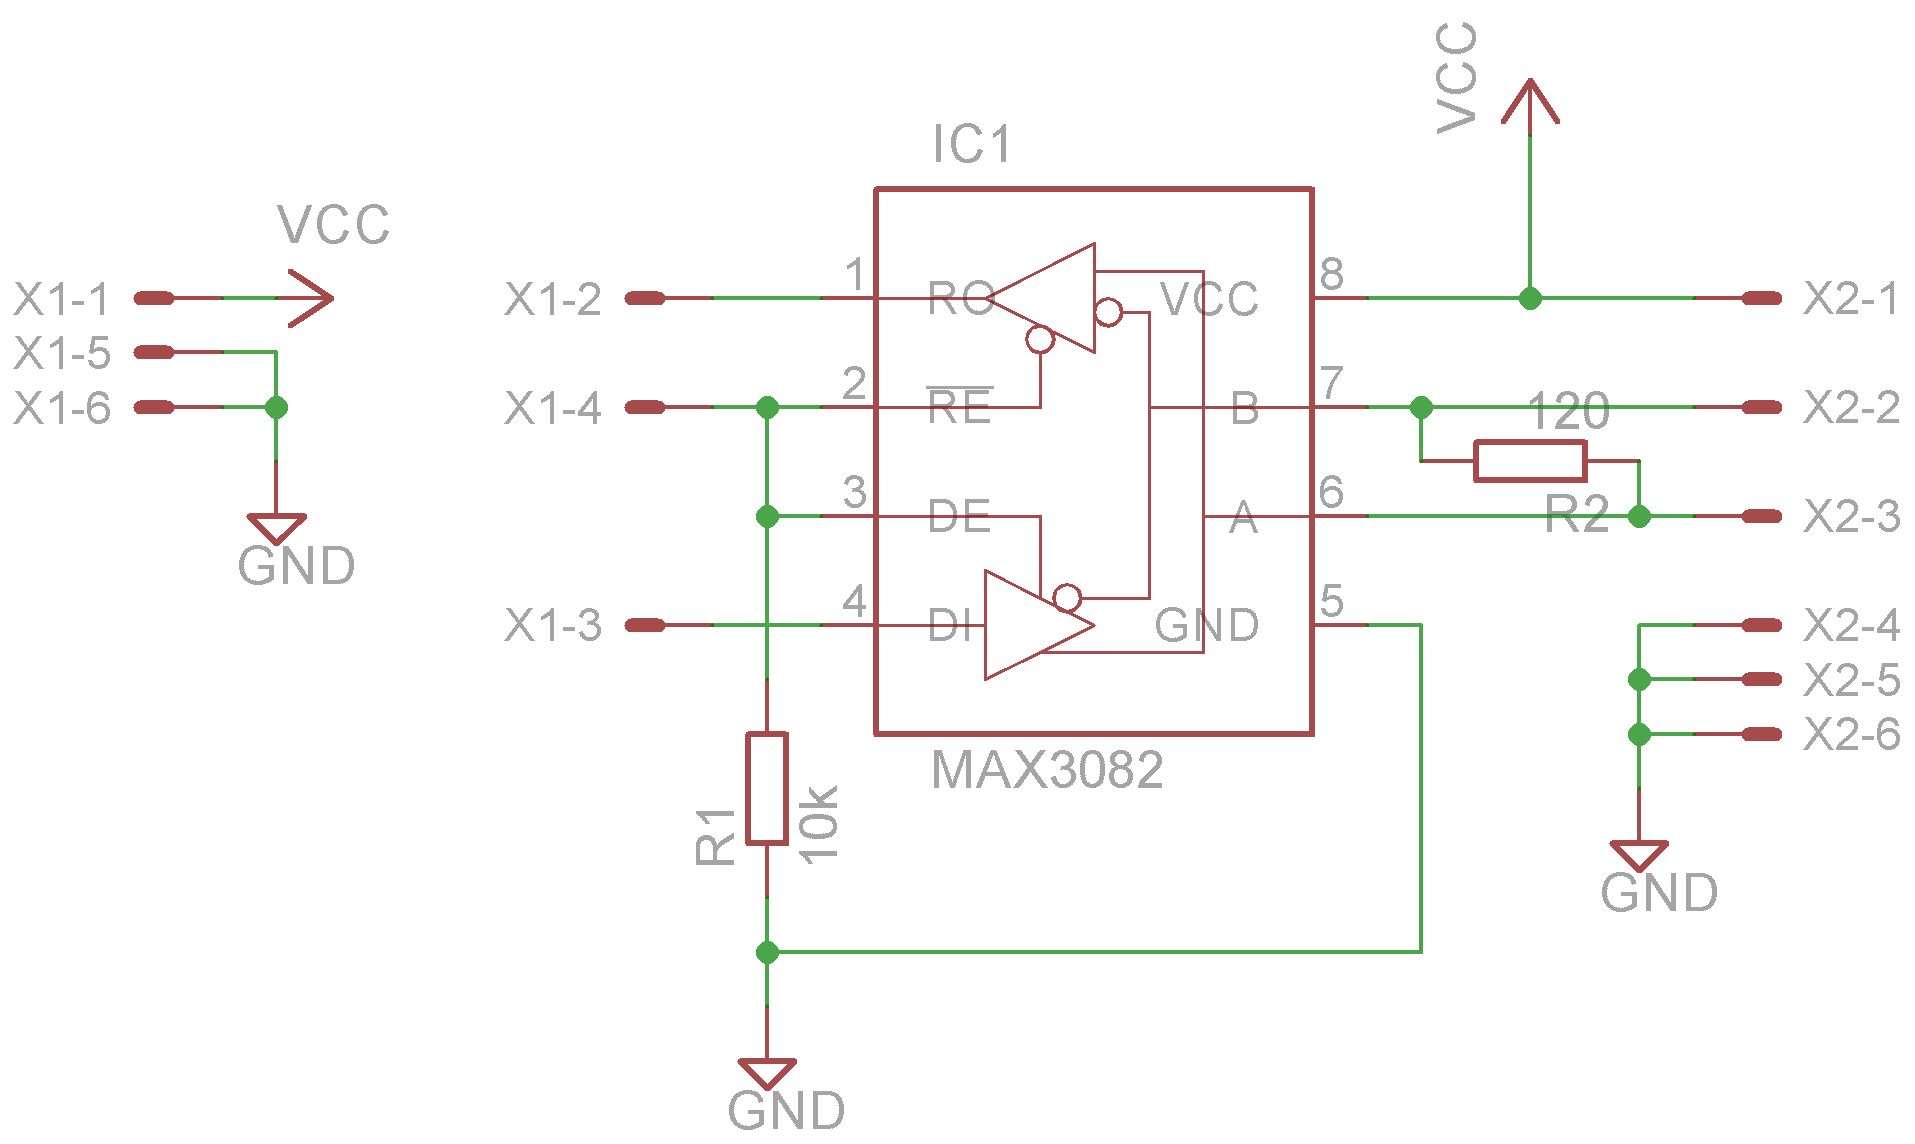
\includegraphics[scale=1]{../Hardware/RS485_Converter/Schematic}
	\caption{RS485 converter}
	\label{photo:RS485converter}
\end{figure}

Bussystemet som er valgt til at kommunikere på er RS485-standarden. Denne beskriver kun de hardwaremæssige krav og det er op til udvikleren selv at lave en protokol. RS485 udmærker sig ved at være en differentiel bus som giver mulighed for at kommunikere over længere afstande (op til 1200m). Der er forbundet arbejde med selv at udvikle en protokol, men det giver også mulighed for at skrue protokollen sådan, at den passer bedst til systemets behov.
\\\\
PSoC4 og Raspberry Pi understøtter dog ikke RS485-kommunikation. De kan begge kommunikere via. RS232/UART. Derfor er der udformet et simpelt RSConverter kredsløb som kan konvertere imellem RS232 og RS485. Kredsløbet benytter sig af MAX3082-kredsen. De eneste eksterne komponenter der er krævet er en pull-down modstand til at trække $TX_{enable}$ lav når den ikke er aktiveret fra PSoC4/Raspberry Pi. Til at terminere buslinjerne kræves en modstand som har samme modstand som det anvendte kabel. Dette gøres for at formindske reflektionen og dermed give det størst mulige signal i modtager-enden.

\subsection{Ventil-/pumpestyring}
Til at styre den valgte pumpe og ventil benyttes et MOSFET-styringskredsløb. 

\begin{figure}[H]
	\centering
	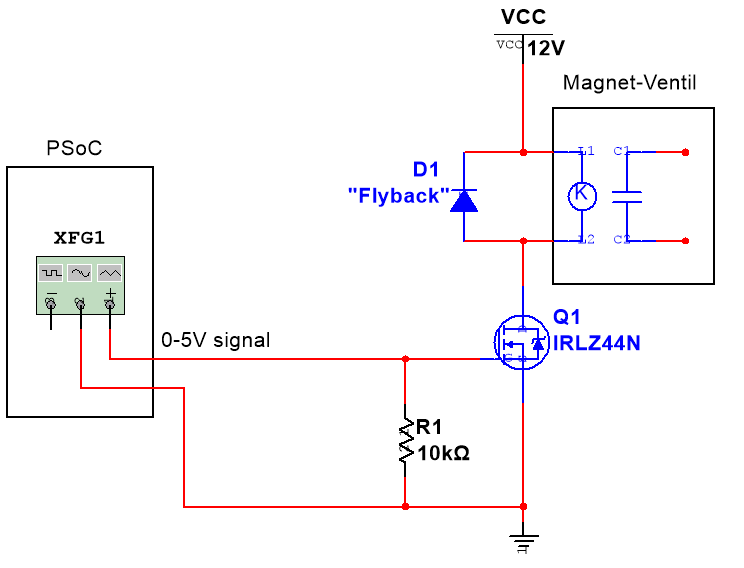
\includegraphics[scale=0.25]{../Hardware/Ventilstyring/Screenshots/VentilStyringskreds}
	\caption{Styringskredsløb til pumpe og ventil}
	\label{screenshot:ventilStyringskreds}
\end{figure}

Begge belastninger optræder som en spole da de indeholder et relæ som skal trækkes. Ved denne form for styring at det vigtigt at notere, at når spændingen fra spolen fjernes, vil den modsætte sig denne ændring ved at skabe en modsatrettet spænding. Denne spænding kan i værste fald beskadige nærsiddende komponenter så kredsløbet ikke længere er funktionelt. Til at modvirke dette benyttes der en såkaldt flyback diode. Derudover benyttes der en pull-down modstand til at trække gaten lav når den ikke er aktiveret af PSoC4'en.

\subsection{Flowsensor}
Når karret skal fyldes med vand er det vigtigt at vide, hvor meget vand der i realiteten er fyldt i karret. Der er valgt en flow sensor til formålet. Jo mere vand som løber igennem sensorer jo højere en frekvens vil den sende ud på udgangen. Dette kræver dog at der over hele tiden som indløbsventilen er åben, konstant holdes øje med signalet den leverer. Dette kræver alt opmærksomhed fra PSoC4'en. 
\\\\
I stedet kan der laves en interrupt som reagere på pulserne fra flowsensoren. Dette vil stadig kræve utrolig meget opmærksomhed fra PSoC4'en. For at fjerne dette problem er der udformet et tæller-kredsløb. Dette kredsløb tæller pulserne fra flowsensoren. Når tælleren ruller over kommer der et interrupt på PSoC4'en. Dette minimerer antallet af interrupts og giver større frihed til PSoC4'en.

\begin{figure}[H]
	\centering
	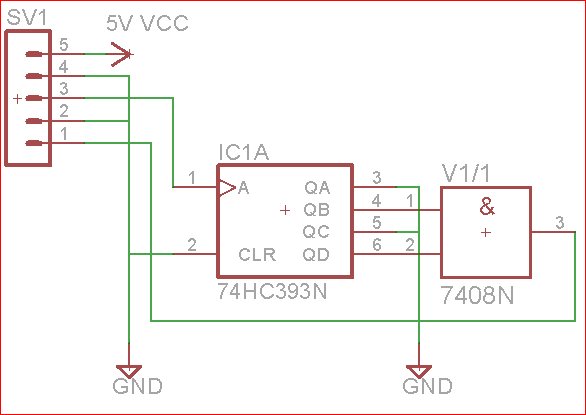
\includegraphics[scale=0.25]{../Hardware/Flow_Sensor/Screenshots/FlowSensor_Schematics_ver1}
	\caption{Counter-kredsløb}
	\label{screenshot:counter}
\end{figure}

Kredsløbet er opbygget omkring en 4-bit tæller (74HC393). Dertil er koblet en AND-gate  som gør, at når tælleren rammer 10 giver den interrupt-signalet til PSoC4'en. Det allerførste der sker i ISR-rutinen er at tælleren nulstilles.

\subsection{Jordfugtsensor}
Planterne kræver at jorden har en hvis jordfugtighed. Dette reguleres ved at vande planterne. For at vide hvornår planterne mangler vand, skal jordfugtigheden måles. Den første idé var at lave en kapacitiv måling. Det viste sig dog ikke at være funktionelt, og idéen blev derfor opgivet.
\\\\
Anden idé var at lave en resistiv måling af jorden. Ved at stikke en 2-benet spyd ned i jorden og sætte 5V over de 2 ben kunne strømmen igennem jorden måles. Udfra dette kan ledningsevnen af jorden beregnes. Det viser sig dog at ved denne målemetode forekommer der en ret kraftig elektrolyse af spydet, som medfører kraftig skade på spydet. Dette kan formindske ved kun at sætte spændingen til spydet når der måles.
\\\\
Forventningen var at ledeevnen af jordet ville stige linæert med jordfugtigheden. Dette viste sig dog i stedet at ligne et fjerdegrads polynomium.

\begin{figure}[H]
	\centering 
	\includegraphics[scale=0.8]{../Projektdokumentation/HardwareArkitektur/Sensore/Jordfugt_billeder/jordspyd.JPG}
	\caption{Diagram over jordspyddet}
	\label{photo:jordspyd_diagram}
\end{figure} 

For at undgå elektrolysen af jordspyddet så meget som muligt, indsættes en MOSFET til at lede strømmen når der skal måles. Modstanden og jordspyddet fungerer som en spændingsdeler. Kondensatoren fungerer som en afkobling for at fjerne evt. støj.

\subsection{pH-probe}
Planterne kræver ikke kun denne rette mændge vand, men også at vandet har den rette pH-værdi. pH-værdien i karret skal derfor måles samtidig med at der doseres gødning i karret. Til denne opgave blev valgt en glasprobe. Det virkede som både den mest effektive men også billigste måde at udføre opgaven på.
\\\\
Glasproben er fyldt med saltsyre og under-/overskud af H+ ioner generer en spænding. For at gøre målingen så præcis som muligt, kræves det er proben kalibreres i en buffer-væske ($pH = 7$) minimum 1 gang om måneden. Første gang systemet startes op skal proben også kalibreres. 
\\\\
I denne måling er der ikke taget højde for, at pH-værdien varierer med temperaturen. Dette ville kræve en temperatur-måling af vandet i karret.
\\\\
Der er foretaget en støjanalyse af proben ud fra den indhentede viden fra E/EP faget MSE (Mixed Signal Elektronik). Analysen viste at det største støjbidrag kom fra støjstrømmen i bufferen. Ved at lave en støjmåling af proben viste det sig at de forventede værdier var ca. en faktor 10 større. Ved høje impedanser blive strømstøjen meget dominerende. Det er derfor meget vigtigt at tage med i sin tanker/beregninger når det endelig kredsløb skal udformes.

\subsection{PSU}
For at forsyne systemet med de rigtige spændingerne og strømme er der udformet en strømforsyning. Den skal tilkobles 230VAC og forsyne systemet med 5V- og 12VDC. Dette kræver en transformering fra 230VAC til 12VAC og 2 reguleringskredsløb. Reguleringskredsløbet til 5V-forsyningen kan ses på figur~\ref{photo:PSU_5V}. Forskellen til 12V-forsyningen er $D_5$ og $R_4$.
 
\begin{figure}[H]
	\centering
	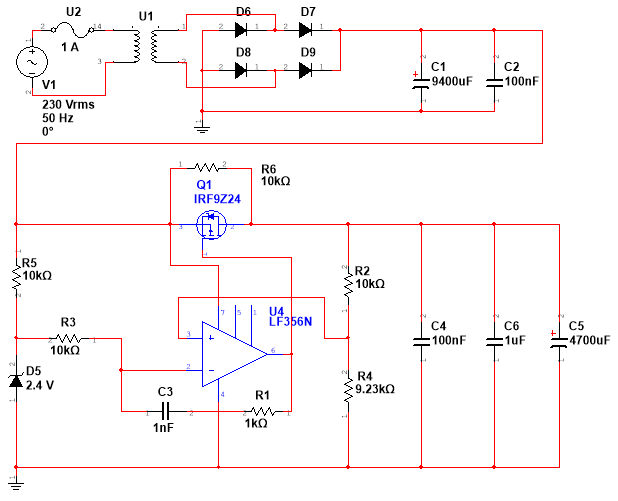
\includegraphics[scale=0.75]{../Hardware/PSU/PSU_5V}
	\caption{5V strømforsynings diagram}
	\label{photo:PSU_5V}
\end{figure}

Spændingen transformeres ned til 12VAC. Spændingen dobbeltensrettes og lades op på nogle store elektrolytter. $D_5$ skaber en reference spænding som fejlforstærkeren kan regulere ud fra. Spændingsdeleren $R_2$ og $R_4$ er udregnet således, at når spændingen på udgangen når over det ønskede punkt, vil fejlforstærkeren lukke for strømgennemløbet i MOSFET'en $Q_1$. For at undgå reguleringsstøj på udgangen er der koblet 2 kondensatorer og 1 elektrolyt på. Samtidig med er forstærkningen i fejlforstærkren gjort frekvens-afhængig hvilket ogsåundertrykker støjens indvirkning på reguleringen.
\\\\
Da der ved fuld belastning afsættes en forholdsvis stor effekt i de 2 regulerings-MOSFETs, er de placeret på en køleplade. 5V-forsyningen trækker en konstant strøm for at forsyne Raspberry Pi, PSoC4 mm. 12V-forsyningen belastes kun når der bruges pumper eller ventiler.

\subsection{Shields til Raspberry og PSoC}
Systemet består af mange små kredsløb og det er derfor valgt at placere alle disse på såkaldte \emph{shields}. Der skal laves 3 forskellige:

\begin{itemize}
\item PiShield
\item Kar-shield
\item Ø-shield
\end{itemize}

Ved at samle kredsløbene på disse \emph{shields} opnår man langt færre ledninger imellem de forskellige blokke. Dette reducerer samtidig med mulighed for støjindlejring fra omverdenen.
\\\\
At udlægge print og teste disse er en forholdsvis stor opgave i forhold til at lave en prototype. Det giver dog et meget bedre overblik over systemet og reducerer muligheden for fejl. Der forekommer også leveringstid på udlagte print og det skaber et endnu større tidspres. Det er dog altid en god idé at designe print sideløbende med at kredsløbene tager form, så det er muligt i f.eks. næste iteration at skabe et fuldt funktionelt system som vil være tæt på det endelige.